\documentclass[xcolor=table]{beamer}
\usetheme{default}
\definecolor{darkscarlet}{rgb}{0.34, 0.01, 0.1}
\usecolortheme{default}
\usecolortheme[named=darkscarlet]{structure}
\setbeamercolor{title}{bg=white, fg=darkscarlet}
\definecolor{cerise}{rgb}{0.87, 0.19, 0.39}
\hypersetup{colorlinks=TRUE,linkcolor=cerise,urlcolor=cerise, citecolor=cerise}

% nummering

\setbeamertemplate{caption}[numbered]

% taal

\usepackage[english]{babel}

% tekens

\usepackage{fontspec}
\usefonttheme{serif}
\setmainfont[BoldFont=brillb.ttf, ItalicFont=brilli.ttf, BoldItalicFont=brillbi.ttf]{brill.ttf}

% tekst doorstrepen, kennelijk heb je daar een apart pakket voor nodig

\usepackage[normalem]{ulem}

% plaatjes

\usepackage{graphicx}

% tabellen

\usepackage{multirow}

% voorbeelden

\usepackage{philex}

% glossen

\usepackage{leipzig}

\newleipzig{hab}{hab}{habitual}
\newleipzig{ad}{ad}{ad}
\newleipzig{el}{el}{elative}
\newleipzig{aor}{aor}{aorist}
\newleipzig{rfl}{rfl}{reflexive}
\newleipzig{emph}{emph}{emphatic particle}
\newleipzig{pf}{pf}{perfect}
\newleipzig{lat}{lat}{lative}
\newleipzig{sup}{sup}{super}
\newleipzig{atr}{atr}{attributivizer}
\newleipzig{add}{add}{additive}
\newleipzig{in}{in}{in}
\newleipzig{rep}{rep}{reportative}
\newleipzig{msd}{msd}{masdar}
\newleipzig{aff}{aff}{affective}
\newleipzig{indef}{indef}{indefinite}
\newleipzig{trans}{trans}{translative}
\newleipzig{an}{an}{animate}
\newleipzig{inan}{inan}{inanimate}
\newleipzig{th}{th}{thematic element}
\newleipzig{ord}{ord}{ordinal numeral}
\newleipzig{temp}{temp}{temporal converb}
\makeglossaries

%\usepackage{natbib}
%\bibpunct[: ]{[}{]}{;}{a}{}{,}

% bibliography

\usepackage[backend=biber,babel=other,
        bibstyle=biblatex-sp-unified,
        citestyle=sp-authoryear-comp,
        doi=false,
        maxcitenames=3,
        maxbibnames=99]{biblatex}
\addbibresource{bibliography.bib}


% custom footline

\setbeamerfont{footline}{size=\fontsize{20}{20}\selectfont}

\newcommand{\Ffootline}{\footnotesize
\insertsection
\hfill
\href{https://github.com/sverhees/2019sle\_ordinals}{github.com/sverhees/2019sle\_ordinals}
\hfill
\insertframenumber/\inserttotalframenumber} 

% custom footline deel 2

\setbeamertemplate{footline}{%
\usebeamerfont{structure}
\begin{beamercolorbox}[wd=\paperwidth,ht=2.25ex,dp=1ex]{title in head/foot}%
\Tiny\hspace*{4mm} \Ffootline \hspace{4mm}
\end{beamercolorbox}}

% navigatiesymbolen uitzetten

\beamertemplatenavigationsymbolsempty
 
 
% titelpagina 

\title{Ordinal numerals and animacy in Botlikh}
\author{Samira Verhees and Chiara Naccarato \\
Linguistic Convergence Laboratory / NRU HSE Moscow}
\date{SLE 21-24.08.2019, Leipzig University}


% links

\usepackage{hyperref}

%\newcommand\pro{\item[$+$]}
%\newcommand\con{\item[$-$]}

\begin{document}

\begin{frame}
\titlepage

\end{frame}

\section{Botlikh}
\begin{frame}{The Botlikh language}

\begin{itemize}
    \item Andic group > East Caucasian language family
    \item Unwritten
    \item \textasciitilde{}5000-8000 speakers
    \item Mostly spoken in 3 villages in Northwestern Daghestan (Russian Federation): Botlikh, Miarso, Ashino. Minor dialectal differences.
    \item One full reference grammar in Georgian  \citep{gudava1962},\footnote{\footnotesize{+ several short sketches mostly repeating the same information.}} one dictionary \citep{saidovaabusov2012} (+ another dictionary in preparation)
\end{itemize}

\end{frame}

\begin{frame}{The Botlikh language}
\begin{itemize}
    \item Opinions vary on the language's vitality --- it is still passed on to children and spoken at home, but some families/children are shifting to Russian
    \item Main village Botlikh is multi-ethnic and mixed marriages are quite common (which is unusual for Daghestan). Avar, Russian and Botlikh are all used for interethnic communication, so there is L2 speaker input into Botlikh and code mixing
\end{itemize}
    
\end{frame}

\section{Gender}
\begin{frame}{Gender agreement: noun class}

\begin{itemize}
    \item Noun class (= gender) agreement system inherited from the proto-language
    \item Semantically transparent assignment
    \item Three classes in singular: \textsc{m} - male humans, \textsc{f} - female humans, \textsc{n} - neuter (residual gender)
    \item Two classes in plural: animates vs. inanimates. (Other EC languages distinguish human vs. non-human in plural.)
\end{itemize}
\end{frame}

\begin{frame}{Gender agreement: noun class}

\begin{table}[H]
\caption{Noun class markers in Botlikh and Godoberi}
\begin{center}
\label{tab:nounclass}
\begin{tabular}{lllllllllll}
   & \textbf{Botlikh} & \textbf{} & \textbf{} & \textbf{} &  &  & \textbf{} & \textbf{Godoberi}   &     &          \\
\textsc{sg} & \textsc{m}                & \textsc{f}         & \textsc{n}         &           &  &  &           & \textsc{m}                   & \textsc{f}   & \textsc{n}        \\
   & w                & j         & b         & b         &  &  &           & w                   & j   & b        \\
\textsc{pl} & \multicolumn{3}{l}{\textsc{an}}                   & \textsc{inan}      &  &  &           & \multicolumn{2}{l}{\textsc{human}} & \textsc{nhuman} \\
   & r/l*             & r/l*      & r/l*      & b         &  &  &           & b                   & b   & r       
\end{tabular}\\
\vspace{0.5cm}
* l is an allomorph that occurs in suffixal position.
\end{center}
\end{table}

\end{frame}

\begin{frame}{Gender agreement: noun class}

Targets include: verbs, adjectives and other attributive forms, inflectional suffixes, postpositions, adverbs, attributivizing clitics.

\pause 

\lb{ex:rope}{\gll hu-\textbf{j} heʔa \textbf{j}-ac'a-rudi ida=χo-\textbf{b} našar go-\textbf{l} wacːilu-di hiƛ'a \textbf{b}-il-o\\
{\Dem}-{\F} up {\F}-reach-{\Temp} {\Cop}={\Atr}-{\N} rope {\Dem}-{\An}.{\Pl} brother.{\Pl}.{\Obl}-{\Erg} down {\N}-throw-{\Aor}\\
\trans `And when she had come up, those brothers threw the rope down.'}

\pause

Attributive forms usually agree with their nominal heads, verbs and other forms agree with an absolutive argument.

\end{frame}

\section{Animacy}
\begin{frame}{Gender agreement: animacy markers}

\begin{itemize}
    \item Additional agreement system for animacy regardless of number
    \item Innovation of Botlikh
    \item Overlaps with the noun class system semantically
    \item Some forms are double marked
\end{itemize}

\end{frame}

\begin{frame}{Gender agreement: animacy markers}

\lb{}{\gll k'eji-\textbf{ɬa-j} ješi\\
two-{\An}.{\Ord}-{\F} girl\\
\trans `the second girl (= daughter)'}

\lb{}{\gll k'eji-\textbf{ɬa-b} zini\\
two-{\An}.{\Ord}-{\N}\\
\trans `the second cow'}

\lb{}{k'eji\textbf{-χo-b} ziw\\
two-{\Inan}.{\Ord}-{\N} day\\
\trans `the second day'}

\end{frame}

\begin{frame}{Gender agreement: animacy markers}

% Animacy markers express agreement by the choice of one of two forms which fulfill another function besides agreement.

% Variety of morphosyntactic constituents derived from the same (lexical?) source

\begin{table}[H]
\caption{Animacy markers in Botlikh}
\begin{center}
\label{tab:animparad}
\begin{tabular}{lll}
\multicolumn{1}{c}{Form} & \multicolumn{1}{c}{Animate} & \multicolumn{1}{c}{Inanimate}                                                      \\ \hline
Negative copula          & ɬi-č'i                      & χu-č'i \\                      
Interrogative particle   & =ɬi.ma                      & =χu.ma \\                  
Question word formant    & =ɬi.la                      & =χu.la \\                  
Attributive clitic       & =ɬa-\textsc{cm}*                     & =χo-\textsc{cm} \\                    
Present participle       & -ɬa-\textsc{cm}*                      & -χa-\textsc{cm} \\
Future participle        & -ɬa-\textsc{cm}*                      & -χo-\textsc{cm} \\
\textbf{> Ordinal numeral}          & -ɬa-\textsc{cm}*                      & -χo-\textsc{cm}
\end{tabular}
\end{center}
\end{table}

*a variant \textit{ɬo-} appears in the environment of the masculine noun class suffix \textit{-w}.

\end{frame}

\begin{frame}{Ordinals}

\begin{itemize}
    \item Based on examples from the dictionary + a small collection of texts (\textasciitilde{}15.000 words, mostly folklore), in the vast majority of cases:
    \item Ordinals agree with their nominal heads
    \item Use is consistent with animate vs. inanimate distinction
    \pause
    \item Speakers mention animacy as the reason for a certain choice 
\end{itemize}

\end{frame}

\section{Ordinals}
\begin{frame}{Ordinals}

Agreement with a controller that is not the nominal head?

\lb{}{\gll \textbf{ištuj-ɬa-b} \textbf{kalasa-ɬi} hiƛ’i w-eχːu\\
five-{\An}.{\Ord}-{\N} grade-{\In} down {\M}-stay.{\Aor}\\
\trans `He stayed \textbf{in the fifth grade} (for another year).’}

\pause

As opposed to:

\lb{}{\gll go-w uškola-ɬi \textbf{hac’aj-χo-b} \textbf{kalasa-ɬi} ida\\
{\Dem}-{\M} school-{\In} ten-{\Inan}.{\Ord}-{\N} grade-{\In} {\Cop}\\
\trans `He is \textbf{in the tenth grade} at school.’}

\end{frame}

\begin{frame}{Ordinals}

Perhaps `grade' is simply an ambiguous word.

\lb{}{\gll ha<r>aža-l kalasːe\\
mix<{\An}.{\Pl}>-{\An}.{\Pl} grade.{\Pl}\\
\trans `mixed grades’}

\pause

Or not...

\lb{}{\gll \textbf{k’eji-ɬa-b} \textbf{reha-di} w-ãʔ-ida w-aƛ’adasisːu-w	waša\\
two-{\An}.{\Ord}-{\N} night-{\Erg} {\M}-go-{\Pf} {\M}-middle-{\M} son\\
`\textbf{On the second night}, the middle son went.'}

\pause

Variation seems possible when the ordinal modifies the head of an adverbial group.

\end{frame}


\section{Survey}
\begin{frame}{Survey}

\begin{center}
Is it possible for the ordinal suffix to agree with something other than its nominal head?\\
\pause
And under which conditions does this occur?
\end{center}

\pause

\begin{itemize}
\item Elicitation task translating from Russian to Botlikh
\item 15 sentences with ordinal numerals (+ 2 sentences with 2 each = 17 questions/stimuli):
\item Modifying an absolutive subject or the head of an adverbial phrase
\item Unambiguously animate / inanimate heads (`daughter', `year') and ambiguous cases
like `grade’ or `family’
\item For each head we had an expectation
\end{itemize}

\end{frame}

\begin{frame}{Results}

\begin{itemize}
\item 13 speakers of Botlikh (+1 from Miarso)
\item Same answer for all speakers in 6/17 questions
\item 24 / 202 unexpected answers were produced (by 9 speakers in 11 questions)\footnote{\footnotesize{Excluding cases where the allomorph \textit{ɬo} appeared instead of \textit{ɬa}. This is possibly a dialectal feature of Ashino.}}
\pause
\item In all cases the animate marker was used where we expected inanimate
\item Heads were known ambiguous nouns (`grade', `family', `people'), and the ordinal was not necessarily in the adverbial group
\end{itemize}
\end{frame}

\begin{frame}{Results}

\begin{figure}[h]
\centering
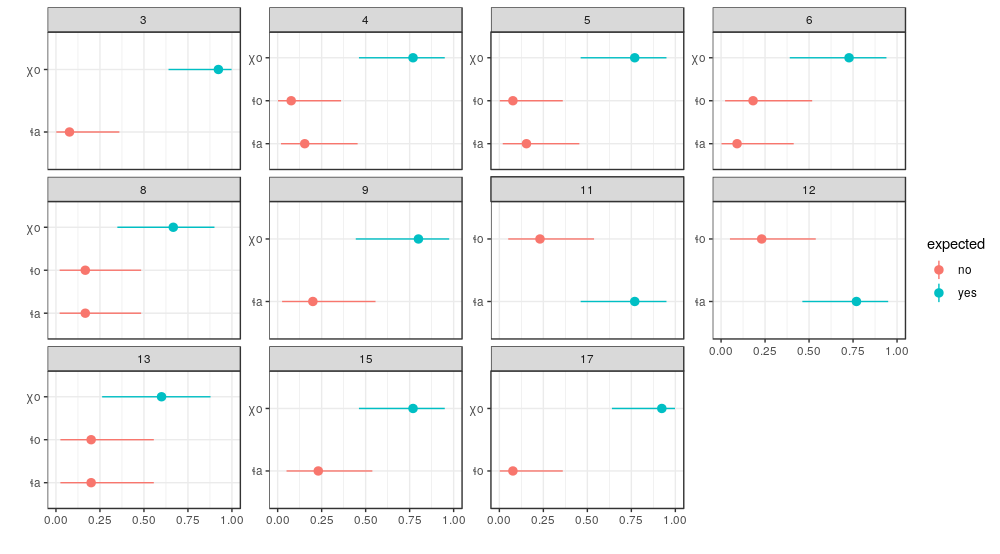
\includegraphics[scale=0.43]{images/ci.png}
\end{figure}
\end{frame}

\begin{frame}{Results}

\begin{itemize}
\item Heads were known ambiguous nouns (`grade', `family', `people'), and the ordinal was not necessarily in the adverbial group
\end{itemize}

\pause

\lb{ex:mount1}{\gll buʁuj-ɬa-b χalq' hãnq'u-di ƛ'ude-χi\\
four-{\An}.{\Ord}-{\N} people house-{\Erg} rock-{\Ad}\\
\trans `The fourth people/nation live in the mountains.'}

\pause

In most cases the noun class marker remained neuter singular, but two speakers used a plural marker.

\pause

\lb{ex:mount1}{\gll buʁuj-ɬa-l χalq' ʕumru ih-u req'-e\\
four-{\An}.{\Ord}-{\An}.{\Pl} people life make-{\Aor} mountain-{\Sup}\\
\trans `The fourth people/nation live in the mountains.'}

\end{frame}

\begin{frame}{Results}

\begin{itemize}
    \item None of the speakers used the animate marker for `year', but four speakers allowed it
    \item Two speakers allowed an inanimate marker with an animate head, each in one specific case. All other speakers unanimously rejected such attempts.
    \item By contrast: the animate form was rejected only 33/97 times where it was not used initially
\end{itemize}

\end{frame}

\begin{frame}{Results}

\centering
\textbf{Side-note} \\
Our Miarso speaker (not taken into account so far) used only the \textit{χo-\textsc{cm}} form, and rejected all my suggestions to rephrase with \textit{ɬa-\textsc{cm}} // \textit{ɬo-\textsc{cm}} saying: ``that's what they say in Botlikh, we don't say that''.
    
\end{frame}

\section{Summary}
\begin{frame}{Summary}
    
    \begin{itemize}
        \item The distribution of ordinal suffixes mostly agrees with the nominal head in terms of animacy
        \item The animate form can appear with typically inanimate heads
        \item In some cases because the heads are ambiguous in terms of animacy, in which case both markers are allowed
        \pause
        \item We do not have an explanation for cases where the animate marker may co-occur with an unambigously inanimate head
        \item It could be a remnant of an old function for the animate marker (e.g. counting vs. singling out, as in Godoberi \citep[241--243]{tatevosov1996})
        \item ... but our survey did not contain many such cases
        \item And we forgot to include animals as heads
    \end{itemize}
\end{frame}


\section*{}

\begin{frame}{Thank you!}

\begin{figure}[h]
\centering
\fbox{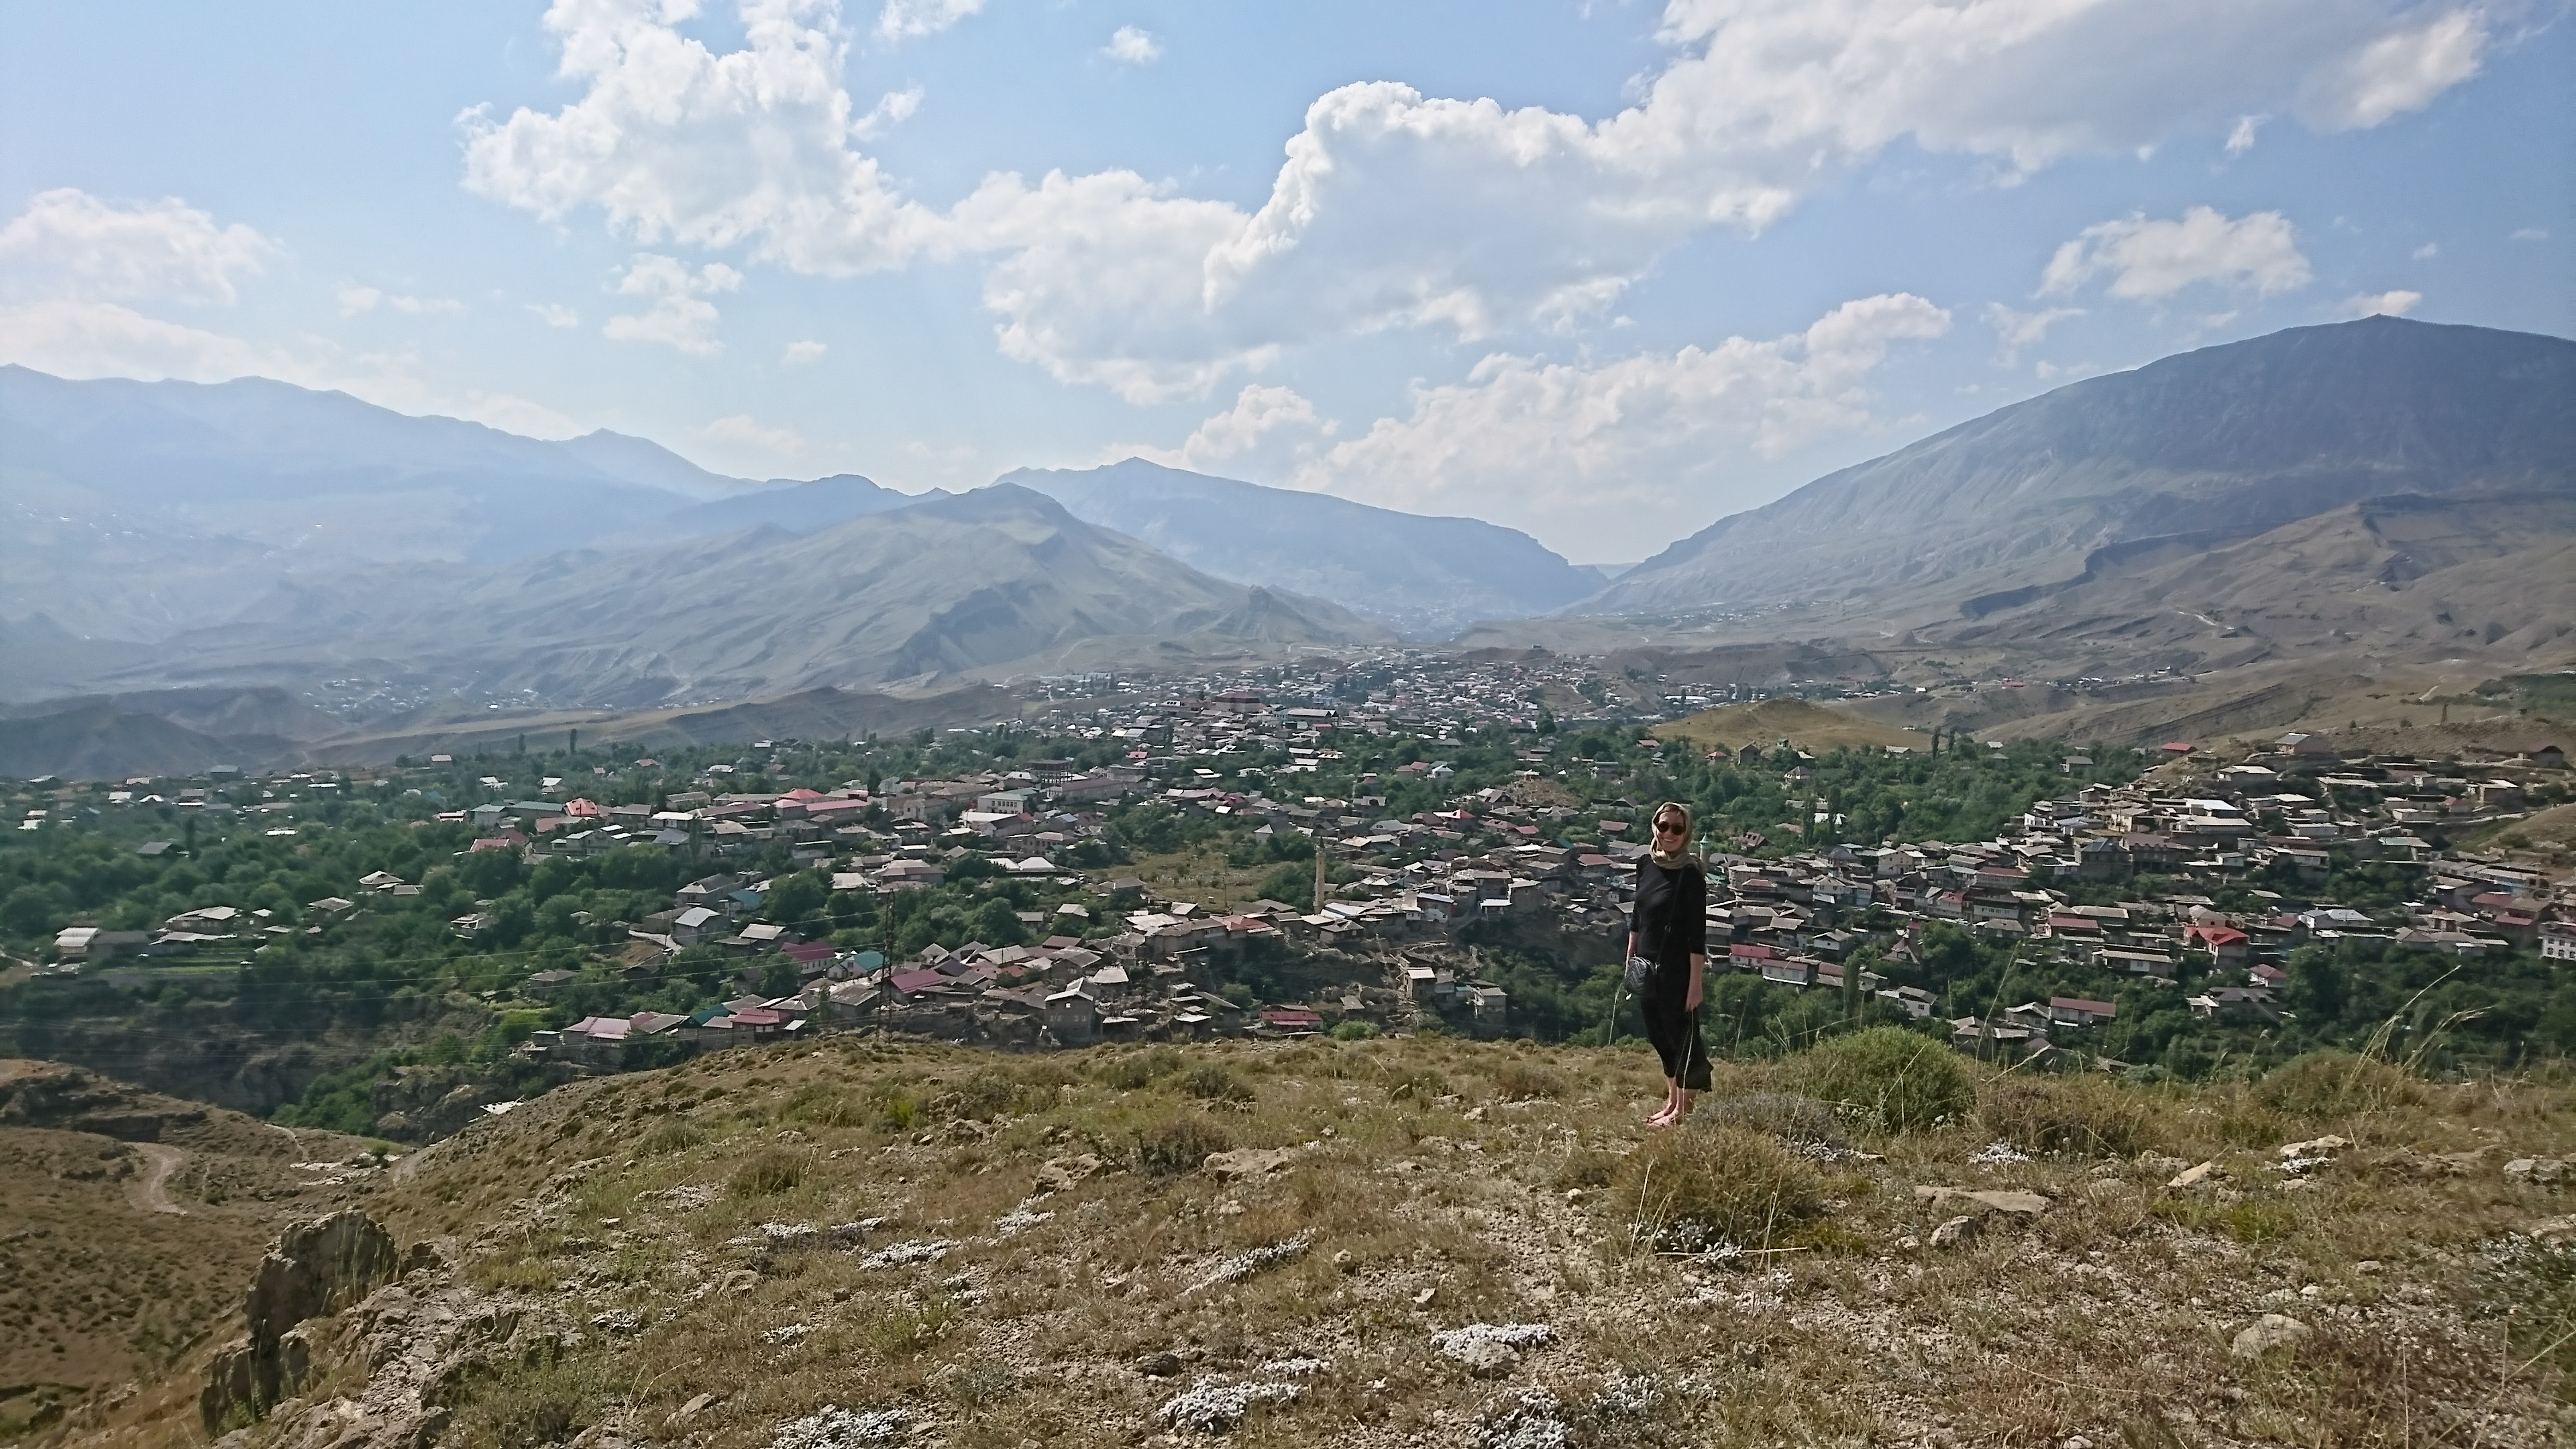
\includegraphics[width=10cm]{images/chiarabotlikh.JPG}}
\end{figure}
    
\end{frame}

\section{Abbreviations}
\begin{frame}{Abbreviations}

\tiny{\printglossary}

\end{frame}

\section{References}
\begin{frame}{References}

\printbibliography

\end{frame}

\end{document}
